\section{Mô hình Khuếch tán (Diffusion Models)}
\label{sec:diffusion_models}

Trong khi GANs thống trị lĩnh vực sinh ảnh trong nhiều năm, chúng vẫn tồn tại những thách thức cố hữu về sự ổn định trong huấn luyện và hiện tượng sụp đổ mode. Vào khoảng năm 2020, một họ mô hình sinh mới, lấy cảm hứng từ nhiệt động lực học, đã nổi lên và nhanh chóng chiếm lĩnh vị trí dẫn đầu: \textbf{Mô hình Khuếch tán (Diffusion Models)}. Với khả năng tạo ra những hình ảnh có chất lượng và sự đa dạng vượt trội, cùng với quá trình huấn luyện ổn định hơn, các mô hình khuếch tán đã mở ra một cuộc cách mạng sáng tạo mới, đặc biệt trong lĩnh vực tạo ảnh từ văn bản.

\subsection{Lý thuyết Cơ bản: Quá trình Khuếch tán và Khử nhiễu}
\label{subsec:diffusion_theory}
Ý tưởng cốt lõi của các mô hình khuếch tán rất thanh lịch:
\begin{enumerate}
	\item Lấy một bức ảnh sạch và từ từ "phá hủy" nó bằng cách thêm nhiễu Gauss từng chút một qua nhiều bước, cho đến khi nó trở thành một mớ nhiễu hoàn toàn. Quá trình này được gọi là \textbf{quá trình thuận (forward process)} hay \textbf{quá trình khuếch tán (diffusion process)}.
	\item Sau đó, huấn luyện một mạng nơ-ron để "đảo ngược" quá trình này: học cách loại bỏ nhiễu một cách từ từ khỏi một ảnh nhiễu hoàn toàn để khôi phục lại một ảnh sạch. Quá trình này được gọi là \textbf{quá trình ngược (reverse process)} hay \textbf{quá trình khử nhiễu (denoising process)}.
\end{enumerate}
Sau khi được huấn luyện, để tạo ra một ảnh mới, chúng ta chỉ cần lấy một mảng nhiễu ngẫu nhiên và cho nó đi qua mạng khử nhiễu này.

\subsubsection{DDPM (Denoising Diffusion Probabilistic Models)}
\label{subsubsec:ddpm}
\textbf{DDPM} \cite{Ho2020} là một công trình nền tảng đã phổ biến hóa và chứng minh hiệu quả của cách tiếp cận này.

\paragraph{Quá trình Thuận (Forward Process):}
Đây là một chuỗi Markov cố định, không cần học. Bắt đầu từ một ảnh sạch $\mathbf{x}_0$, ở mỗi bước thời gian $t$, chúng ta thêm một lượng nhỏ nhiễu Gauss để tạo ra $\mathbf{x}_t$:
\begin{equation}
	q(\mathbf{x}_t | \mathbf{x}_{t-1}) = \mathcal{N}(\mathbf{x}_t; \sqrt{1 - \beta_t} \mathbf{x}_{t-1}, \beta_t \mathbf{I})
\end{equation}
trong đó $\{\beta_t\}_{t=1}^T$ là một \textbf{lịch trình phương sai (variance schedule)} được định nghĩa trước, thường là các giá trị nhỏ tăng dần. Một thuộc tính quan trọng của quá trình này là chúng ta có thể lấy mẫu $\mathbf{x}_t$ trực tiếp từ $\mathbf{x}_0$ ở bất kỳ bước nào:
\begin{equation}
	\mathbf{x}_t = \sqrt{\bar{\alpha}_t} \mathbf{x}_0 + \sqrt{1 - \bar{\alpha}_t} \boldsymbol{\epsilon}
	\label{eq:ddpm_forward_direct}
\end{equation}
với $\alpha_t = 1 - \beta_t$, $\bar{\alpha}_t = \prod_{i=1}^t \alpha_i$, và $\boldsymbol{\epsilon} \sim \mathcal{N}(\mathbf{0}, \mathbf{I})$. Khi $T$ đủ lớn (ví dụ: 1000), $\bar{\alpha}_T \approx 0$, và $\mathbf{x}_T$ sẽ gần như là nhiễu chuẩn.

\paragraph{Quá trình Ngược (Reverse Process):}
Đây là phần có thể học được. Mục tiêu là học một mạng nơ-ron $\boldsymbol{\epsilon}_\theta(\mathbf{x}_t, t)$ để \textbf{dự đoán nhiễu $\boldsymbol{\epsilon}$} đã được thêm vào ảnh ở bước $t$.
\begin{itemize}
	\item \textbf{Kiến trúc:} Mạng này thường là một kiến trúc U-Net, với các cơ chế self-attention được thêm vào để xử lý thông tin toàn cục. Nó nhận đầu vào là ảnh nhiễu $\mathbf{x}_t$ và bước thời gian $t$ (thường được mã hóa bằng positional encoding).
	\item \textbf{Hàm mất mát:} Hàm mất mát được đơn giản hóa một cách đáng kinh ngạc. Tại mỗi bước huấn luyện, chúng ta:
	\begin{enumerate}
		\item Lấy một ảnh sạch $\mathbf{x}_0$.
		\item Chọn một bước thời gian ngẫu nhiên $t \in [1, T]$.
		\item Tạo một mẫu nhiễu ngẫu nhiên $\boldsymbol{\epsilon} \sim \mathcal{N}(\mathbf{0}, \mathbf{I})$.
		\item Tạo ảnh nhiễu $\mathbf{x}_t$ bằng công thức \ref{eq:ddpm_forward_direct}.
		\item Yêu cầu mạng dự đoán nhiễu $\boldsymbol{\epsilon}$ từ $\mathbf{x}_t$.
	\end{enumerate}
	Hàm mất mát chỉ đơn giản là Mean Squared Error (MSE) giữa nhiễu thật và nhiễu được dự đoán:
	\begin{equation}
		\mathcal{L}_{\text{simple}} = \mathbb{E}_{t, \mathbf{x}_0, \boldsymbol{\epsilon}} \left[ ||\boldsymbol{\epsilon} - \boldsymbol{\epsilon}_\theta(\sqrt{\bar{\alpha}_t} \mathbf{x}_0 + \sqrt{1 - \bar{\alpha}_t} \boldsymbol{\epsilon}, t)||^2 \right]
	\end{equation}
\end{itemize}

\begin{center}
	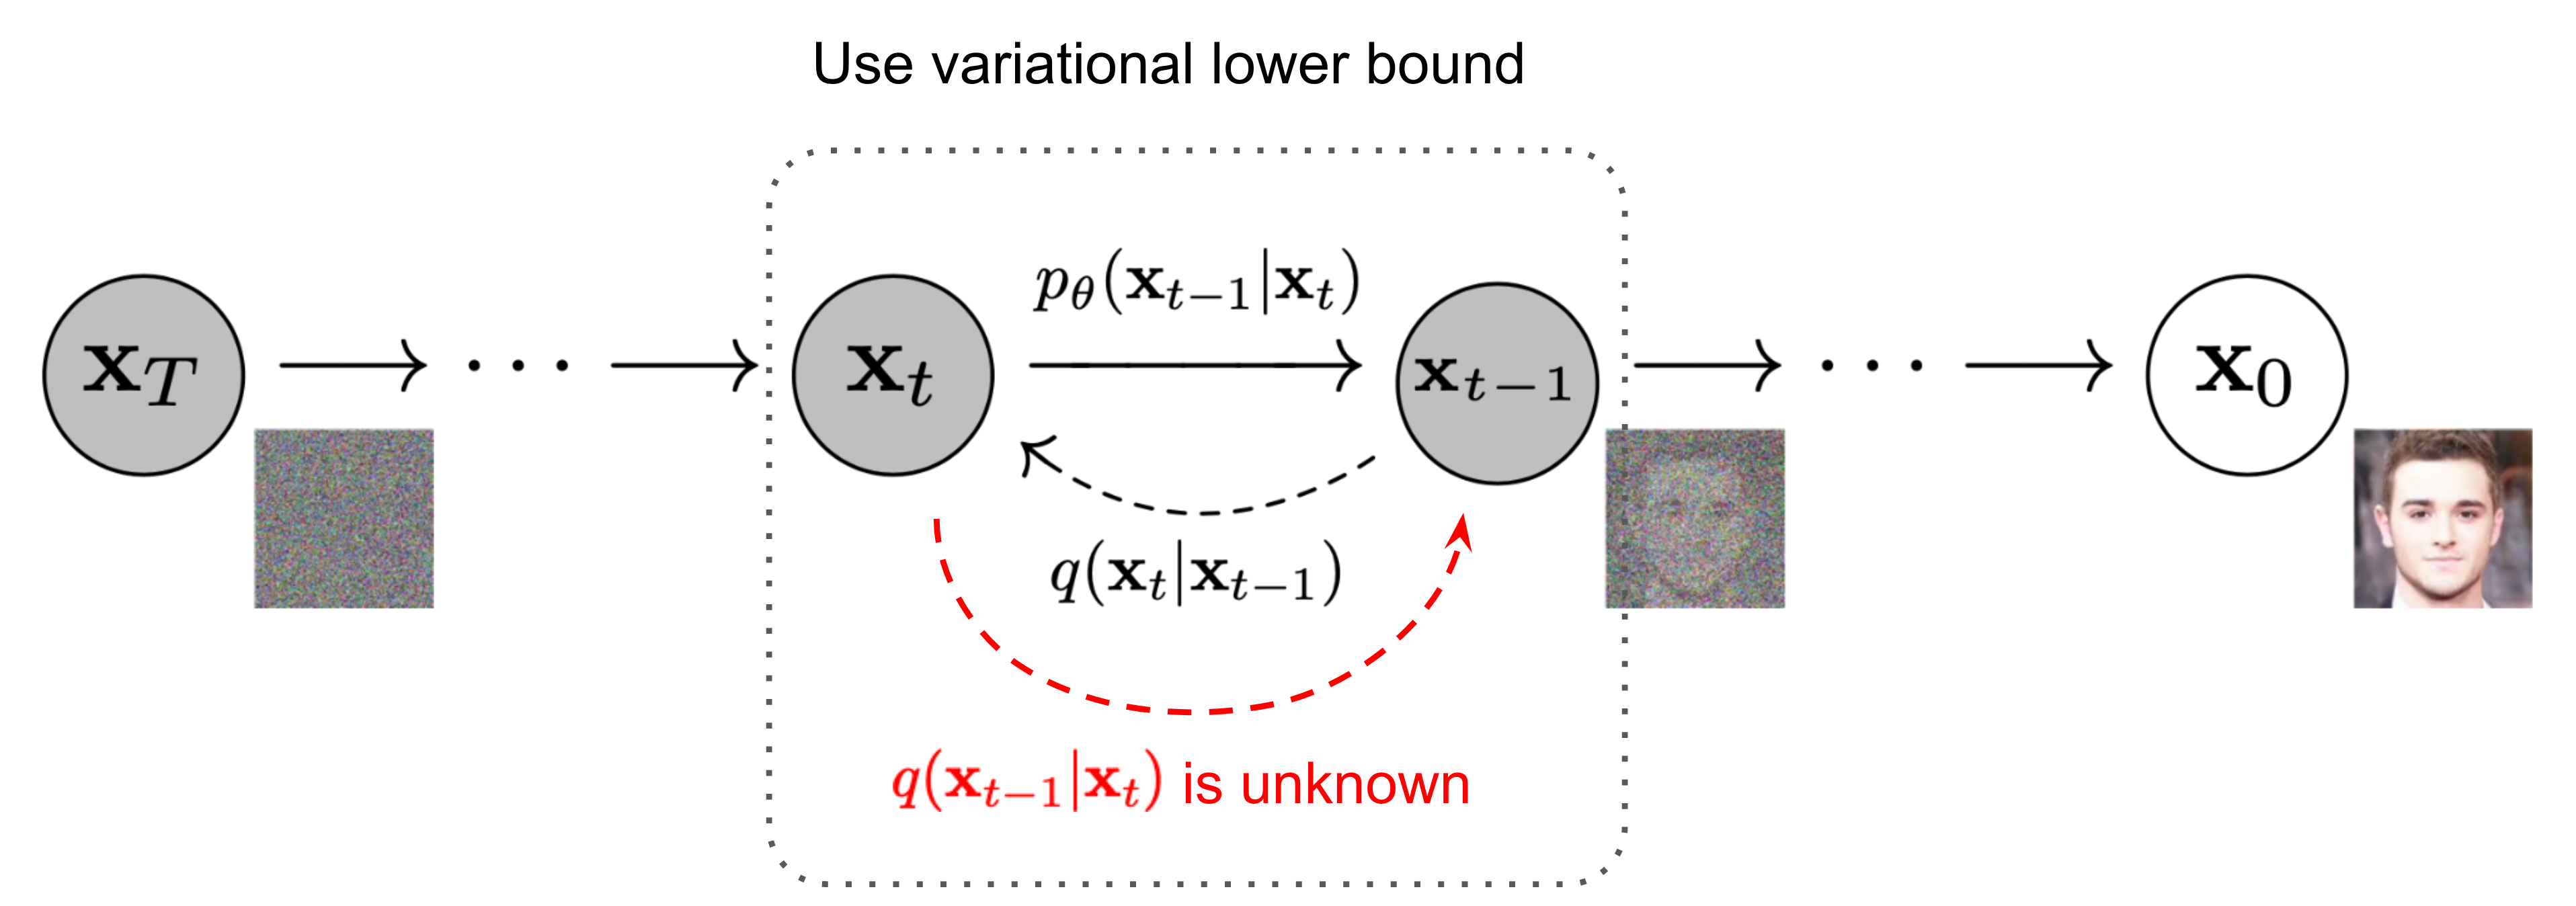
\includegraphics[width=1.0\textwidth]{images/ddpm_diffusion_process.png}
	\captionof{figure}{Minh họa quá trình khuếch tán. Quá trình thuận (trên) dần dần thêm nhiễu vào ảnh. Quá trình ngược (dưới) sử dụng một mạng U-Net để học cách khử nhiễu từng bước một, bắt đầu từ nhiễu thuần túy.}
	\label{fig:ddpm_process}
\end{center}
% Keyword gợi ý: ddpm diffusion process, denoising diffusion probabilistic models

\textbf{Quá trình Lấy mẫu (Sampling):} Sau khi huấn luyện, để tạo ảnh mới, chúng ta bắt đầu với một nhiễu ngẫu nhiên $\mathbf{x}_T \sim \mathcal{N}(\mathbf{0}, \mathbf{I})$ và lặp lại quá trình khử nhiễu từ $t=T$ về $1$, sử dụng nhiễu đã dự đoán để ước tính $\mathbf{x}_{t-1}$.

\subsection{Latent Diffusion và Stable Diffusion: Hiệu quả trong Không gian Tiềm ẩn}
\label{subsec:latent_diffusion}

Một nhược điểm lớn của các mô hình khuếch tán gốc như DDPM là chúng hoạt động trực tiếp trên không gian pixel có chiều rất cao, dẫn đến:
\begin{itemize}
	\item Quá trình huấn luyện tốn nhiều GPU/TPU.
	\item Quá trình sinh ảnh (sampling) chậm vì phải thực hiện hàng trăm đến hàng nghìn bước khử nhiễu.
\end{itemize}

\textbf{Latent Diffusion Models (LDM)} \cite{Rombach2022}, nền tảng của \textbf{Stable Diffusion}, giải quyết vấn đề này bằng cách thực hiện khuếch tán trong một không gian tiềm ẩn có chiều thấp hơn nhiều.

\begin{itemize}
	\item \textbf{Ý tưởng chính:} Thay vì áp dụng quá trình diffusion trực tiếp trên ảnh $\mathbf{x}$, ta thực hiện trên biểu diễn tiềm ẩn $\mathbf{z} = \mathcal{E}(\mathbf{x})$, giúp giảm chiều dữ liệu và tốc độ tính toán.
	
	\item \textbf{Kiến trúc chính của LDM:}
	\begin{enumerate}
		\item \textbf{Autoencoder (VAE):} 
		\begin{itemize}
			\item Encoder $\mathcal{E}$ nén ảnh gốc $\mathbf{x}$ thành biểu diễn tiềm ẩn $\mathbf{z}$.
			\item Decoder $\mathcal{D}$ tái tạo ảnh từ biểu diễn $\mathbf{z}$: $\mathbf{x} \approx \mathcal{D}(\mathbf{z})$.
			\item Không gian tiềm ẩn này thường nhỏ hơn 8–16 lần so với ảnh gốc về cả chiều không gian và kênh.
		\end{itemize}
		
		\item \textbf{Diffusion Model (U-Net):} 
		\begin{itemize}
			\item Quá trình khuếch tán (forward diffusion) và khử nhiễu (reverse diffusion) diễn ra trên $\mathbf{z}$ thay vì $\mathbf{x}$.
			\item Mạng U-Net học để dự đoán noise hoặc residual trong không gian tiềm ẩn.
			\item Giảm đáng kể số lượng phép tính so với diffusion trực tiếp trên pixel.
		\end{itemize}
		
		\item \textbf{Conditioning Mechanism:} 
		\begin{itemize}
			\item Nhúng thông tin điều kiện (ví dụ: văn bản) thông qua cross-attention vào U-Net.
			\item Text encoder (thường là CLIP) chuyển chuỗi văn bản thành embedding $\mathbf{c}$.
			\item U-Net sử dụng $\mathbf{c}$ để điều khiển quá trình sinh ảnh theo nội dung mô tả.
		\end{itemize}
	\end{enumerate}
\end{itemize}

\textbf{Lợi ích:}
\begin{itemize}
	\item Tốc độ sinh ảnh nhanh hơn nhiều nhờ giảm chiều không gian.
	\item Dễ dàng tạo ảnh độ phân giải cao.
	\item Khả năng điều khiển sinh ảnh bằng nhiều loại điều kiện khác nhau (text, segmentation, depth maps,...).
\end{itemize}

\textbf{Stable Diffusion:} Là phiên bản LDM được huấn luyện trên quy mô lớn với các bộ dữ liệu đa dạng và phát hành dưới dạng mã nguồn mở, trở thành công cụ phổ biến trong cộng đồng AI sáng tạo để sinh ảnh theo văn bản, chỉnh sửa ảnh, và nhiều ứng dụng sáng tạo khác.

\begin{center}
	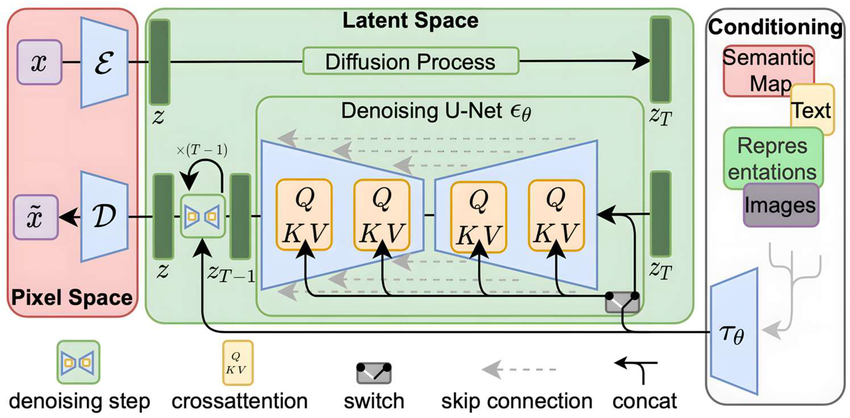
\includegraphics[width=0.95\textwidth]{images/stable_diffusion_pipeline.png}
	\captionof{figure}{Pipeline của Latent Diffusion Model (LDM) và Stable Diffusion. Ảnh gốc được mã hóa vào không gian tiềm ẩn, diffusion thực hiện trên latent space với điều kiện văn bản, và decoder tái tạo ảnh cuối cùng.}
	\label{fig:latent_diffusion_pipeline}
\end{center}
% Keyword gợi ý: latent diffusion model, stable diffusion, LDM architecture
\subsection{Kỹ thuật Điều khiển Quá trình Sinh ảnh}
\label{subsec:diffusion_control_techniques}

Sức mạnh thực sự của các mô hình khuếch tán không chỉ nằm ở khả năng tạo ra các ảnh ngẫu nhiên chất lượng cao, mà còn ở khả năng kiểm soát và tùy chỉnh quá trình sinh một cách tinh vi. Nhiều kỹ thuật gần đây cho phép chúng ta điều khiển nội dung, bố cục, phong cách, và thậm chí là các đối tượng cụ thể trong ảnh.

\begin{description}
	\item[Textual Inversion:] \cite{Gal2022_textual} 
	\begin{itemize}
		\item \textbf{Mục tiêu:} Cho phép mô hình học một khái niệm thị giác mới từ chỉ một vài (3-5) bức ảnh, mà không cần huấn luyện lại toàn bộ mô hình.
		\item \textbf{Cơ chế:} 
		\begin{enumerate}
			\item Giữ "đóng băng" toàn bộ mô hình diffusion và text encoder.
			\item Tối ưu hóa một embedding vector mới trong từ vựng của text encoder, ví dụ `S*`.
			\item Vector `S*` có thể được dùng trong prompt như một từ khóa: \textit{"a photo of S* in the style of Van Gogh"}.
		\end{enumerate}
		\item \textbf{Ưu điểm:} Nhanh, tiết kiệm tài nguyên, dễ tích hợp vào pipeline hiện có.
		\item \textbf{Hạn chế:} Khả năng tạo ra các chi tiết phức tạp hoặc phong cách đặc trưng đôi khi kém hơn các phương pháp fine-tune.
	\end{itemize}
	
	\item[DreamBooth:] \cite{Ruiz2023_dreambooth}
	\begin{itemize}
		\item \textbf{Mục tiêu:} Cá nhân hóa mô hình diffusion để sinh ra các đối tượng hoặc phong cách cụ thể với độ chính xác cao.
		\item \textbf{Cơ chế:} 
		\begin{enumerate}
			\item Thay vì chỉ học một embedding, DreamBooth tinh chỉnh một phần nhỏ của toàn bộ U-Net.
			\item Sử dụng một định danh lớp hiếm (rare class token), ví dụ `sks`, để tránh quên các khái niệm gốc: \textit{"a photo of a sks dog"}.
			\item Kết hợp dữ liệu ảnh mới của đối tượng với prompt để mô hình học cả nội dung và phong cách đặc trưng.
		\end{enumerate}
		\item \textbf{Ưu điểm:} Tạo ảnh cá nhân hóa rất chính xác, duy trì các chi tiết đặc trưng của đối tượng.
		\item \textbf{Hạn chế:} Yêu cầu nhiều tài nguyên hơn so với Textual Inversion và quá trình fine-tune cần cẩn trọng để tránh "overfitting".
	\end{itemize}
	
	\item[ControlNet:] \cite{Zhang2023_controlnet}
	\begin{itemize}
		\item \textbf{Mục tiêu:} Tăng khả năng điều khiển chi tiết quá trình sinh ảnh bằng các điều kiện không gian như đường viền (edges), tư thế (pose), độ sâu (depth map) hoặc phác thảo (scribbles).
		\item \textbf{Kiến trúc:} 
		\begin{enumerate}
			\item Đóng băng toàn bộ mô hình diffusion lớn đã được huấn luyện trước (như Stable Diffusion).
			\item Tạo một bản sao của các khối mã hóa trong mô hình gốc và huấn luyện bản sao này (gọi là "ControlNet") để nhận thêm đầu vào điều kiện.
			\item Output từ ControlNet được cộng vào output của các lớp tương ứng trong mô hình diffusion gốc, "hướng dẫn" quá trình khử nhiễu theo cấu trúc mong muốn.
		\end{enumerate}
		\item \textbf{Quá trình hoạt động:} 
		\begin{itemize}
			\item Nhập ảnh điều kiện (ví dụ: skeleton pose, edge map) vào ControlNet.
			\item ControlNet điều chỉnh các đặc trưng trong quá trình diffusion, đảm bảo ảnh sinh ra tuân theo bố cục/chi tiết của điều kiện.
		\end{itemize}
		\item \textbf{Ưu điểm:} 
		\begin{itemize}
			\item Cho phép kiểm soát chính xác bố cục, tư thế, và các chi tiết hình học.
			\item Dễ kết hợp với các kỹ thuật điều kiện khác như Text-to-Image hoặc DreamBooth.
		\end{itemize}
		\item \textbf{Hạn chế:} Yêu cầu ảnh điều kiện phù hợp và đôi khi tăng chi phí tính toán.
	\end{itemize}
\end{description}

\begin{center}
	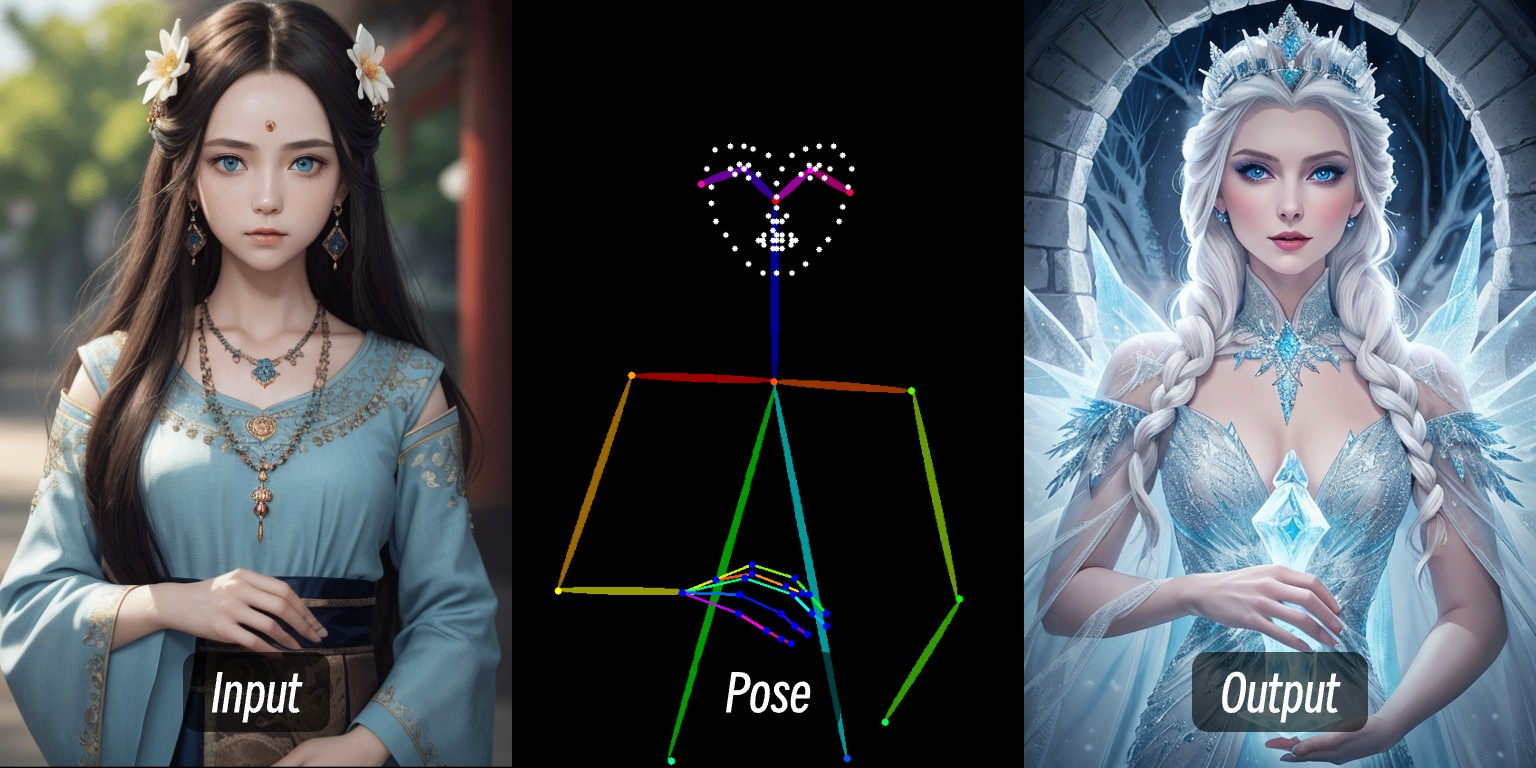
\includegraphics[width=1.0\textwidth]{images/controlnet_pose_example.jpg}
	\captionof{figure}{Ví dụ về ControlNet: bằng cách cung cấp một ảnh tư thế (pose) làm điều kiện, ControlNet hướng dẫn mô hình diffusion (Stable Diffusion) tạo ra nhân vật với tư thế chính xác.}
	\label{fig:controlnet_example}
\end{center}

\subsection{Kết luận: Một Kỷ nguyên Mới của Sáng tạo Thị giác}
\label{subsec:diffusion_conclusion}
Các mô hình khuếch tán đã thay đổi cuộc chơi trong lĩnh vực AI sáng tạo. Chúng không chỉ vượt qua GANs về chất lượng và sự đa dạng của ảnh sinh ra, mà còn cung cấp một nền tảng ổn định và cực kỳ linh hoạt để điều khiển quá trình sáng tạo.

Từ nền tảng lý thuyết của DDPM, sự tối ưu hóa hiệu quả của Latent Diffusion, đến khả năng kiểm soát tinh vi của ControlNet, DreamBooth, và Textual Inversion, các mô hình khuếch tán đã dân chủ hóa khả năng sáng tạo nghệ thuật, biến những ý tưởng trong văn bản thành những tác phẩm thị giác chi tiết. Chúng là công nghệ cốt lõi đằng sau cuộc cách mạng text-to-image và đang nhanh chóng được mở rộng sang các lĩnh vực video, 3D, và âm thanh, hứa hẹn một tương lai nơi ranh giới giữa trí tưởng tượng của con người và khả năng tổng hợp của máy móc ngày càng bị xóa nhòa.

\section*{Tài liệu tham khảo}
\begin{itemize}
	\item[1] Ho, J., Jain, A., \& Abbeel, P. (2020). Denoising diffusion probabilistic models. In \textit{Advances in Neural Information Processing Systems (NeurIPS)}. (Paper gốc giới thiệu DDPM).
	\item[2] Rombach, R., Blattmann, A., Lorenz, D., Esser, P., \& Ommer, B. (2022). High-resolution image synthesis with latent diffusion models. In \textit{Proceedings of the IEEE/CVF Conference on Computer Vision and Pattern Recognition (CVPR)}. (Paper gốc giới thiệu Latent Diffusion Models, nền tảng của Stable Diffusion).
	\item[3] Zhang, L., \& Agrawala, M. (2023). Adding conditional control to text-to-image diffusion models. In \textit{Proceedings of the IEEE/CVF International Conference on Computer Vision (ICCV)}. (Paper gốc giới thiệu ControlNet).
	\item[4] Gal, R., Alaluf, Y., Atzmon, Y., Patashnik, O., Bermano, A. H., \& Cohen-Or, D. (2022). An image is worth one word: Personalizing text-to-image generation using textual inversion. In \textit{ECCV Workshops}. (Paper gốc giới thiệu Textual Inversion).
	\item[5] Ruiz, N., Li, Y., Jampani, V., Pritch, Y., Rubinstein, M., \& Aberman, K. (2023). Dreambooth: Fine-tuning text-to-image diffusion models for subject-driven generation. In \textit{Proceedings of the IEEE/CVF Conference on Computer Vision and Pattern Recognition (CVPR)}. (Paper gốc giới thiệu DreamBooth).
	\item[6] Sohl-Dickstein, J., Weiss, E., Maheswaranathan, N., \& Ganguli, S. (2015). Deep unsupervised learning using nonequilibrium thermodynamics. In \textit{International Conference on Machine Learning (ICML)}. (Một trong những công trình lý thuyết sơ khai đặt nền móng cho các mô hình khuếch tán).
\end{itemize}